\documentclass[zihao=-4,a4paper,UTF8,fontset=windows]{ctexart}
\usepackage[top=2.5cm,bottom=2.5cm,left=3cm,right=3cm,headheight=0.9cm,headsep=0.58cm,footskip=1.23cm]{geometry}
\usepackage{fancyhdr}
\usepackage{longtable}
\usepackage{array}
\usepackage{graphicx}
\usepackage{xcolor}
\usepackage{enumitem}
\definecolor{aicblue}{RGB}{18,86,184}
\pagestyle{fancy}
\fancyhf{}
\fancyhead[L]{
\includegraphics[height=0.55cm]{aic_logo.png}}
\fancyhead[R]{\zihao{-5} 2026 第八届全球校园人工智能算法精英大赛}
\renewcommand{\headrulewidth}{0.5pt}
\fancyfoot[C]{\zihao{5}\thepage}
% 封面页样式：页眉同正文（官方 logo + 大赛名），页脚无页码（对照官方模板封面）
\fancypagestyle{cover}{%
  \fancyhf{}%
  \fancyhead[L]{
\includegraphics[height=0.55cm]{aic_logo.png}}%
  \fancyhead[R]{\zihao{-5} 2026 第八届全球校园人工智能算法精英大赛}%
  \renewcommand{\headrulewidth}{0.5pt}%
  \fancyfoot[C]{}%
}
% 列表符号用中文间隔号（降 AI 味，不用英文圆点）
\renewcommand{\labelitemi}{\textperiodcentered}
\renewcommand{\labelitemii}{--}
% 标题层级：一级三号粗体 / 二级四号粗体 / 三级小四粗体（模板规范）
% 标题字体：宋体加粗（官方格式清单：一二三级标题均宋体粗体），字号 三号/四号/小四
\setcounter{secnumdepth}{-1}
\usepackage{titlesec}
\titleformat{\section}{\bfseries\zihao{3}}{}{0em}{}
\titleformat{\subsection}{\bfseries\zihao{4}}{}{0em}{}
\titleformat{\subsubsection}{\bfseries\zihao{-4}}{}{0em}{}
\titlespacing*{\section}{0pt}{1.2em}{0.6em}
\titlespacing*{\subsection}{0pt}{0.8em}{0.4em}
\titlespacing*{\subsubsection}{0pt}{0.6em}{0.3em}
% 西文 Times New Roman（fontspec）
\usepackage{fontspec}
\setmainfont{Times New Roman}
% 中文主字体宋体，粗体走 XeLaTeX 仿粗（对应 Word 的"宋体+加粗"，官方格式清单）
\setCJKmainfont[AutoFakeBold=3]{SimSun}
% 带圈数字①-⑳等符号区字符用中文字体渲染（Times 无字形，否则出豆腐块）
\xeCJKDeclareCharClass{CJK}{"2460 -> "24FF}
% 标题孤行控制：页尾不足三行时不排标题
\usepackage{needspace}
\newcommand{\sectionbreak}{\needspace{3\baselineskip}}
\newcommand{\subsectionbreak}{\needspace{3\baselineskip}}
\newcommand{\subsubsectionbreak}{\needspace{3\baselineskip}}
% 行距：单倍（Word 宋体小四单倍 = 12pt × 1.3 ≈ 15.6pt；ctex 基准 baselineskip 14.4pt，1.083 × 14.4 ≈ 15.6）
\linespread{1.083}
\setlength{\parindent}{2em}
% 标题后的首段也缩进（中文排版惯例，模板正文全部段首空两格）
\usepackage{indentfirst}
\setlength{\parskip}{0pt}
\renewcommand{\arraystretch}{1.15}
\begin{document}
% ===== 封面 =====（对照官方模板：标题群上 1/4 起、团队信息中部左对齐下划线、日期底部、无页码）
\begin{titlepage}
\thispagestyle{cover}
\vspace*{2.8cm}
\begin{center}
{\bfseries\zihao{1} 2026 年第八届}\\[0.8em]
{\bfseries\zihao{1} 全球校园人工智能算法精英大赛}\\[3em]
{\bfseries\zihao{3} 算法创新赛}\\[1em]
{\bfseries\zihao{3}（AI+学科交叉）}\\[1em]
{\bfseries\zihao{3} 技术报告}\\
\end{center}
\vspace{5em}
\begin{flushleft}
\hspace*{4em}\zihao{4}
团队名称：\underline{\makebox[7cm][c]{一起搞事情}}\\[0.8em]
\hspace*{4em}参赛编号：\underline{\makebox[7cm][c]{AIC-2026-21740176}}\\[0.8em]
\hspace*{4em}作品名称：\underline{\makebox[7cm][c]{LearnLab 跨学科智能学习平台}}\\
\end{flushleft}
\vfill
\begin{center}\zihao{4} 日期：2026 年 10 月\end{center}
\vspace*{1.5cm}
\end{titlepage}
\setcounter{page}{1}
% ===== 目录 =====（目录标题：宋体二号粗体居中——官方格式清单；条目格式不受影响）
\begingroup
\titleformat{\section}{\centering\bfseries\zihao{2}}{}{0em}{}
\renewcommand{\contentsname}{目\quad 录}
\setcounter{tocdepth}{3}
\tableofcontents
\endgroup
\newpage
% ===== 作品简介 =====
\section*{作品简介}
\addcontentsline{toc}{section}{作品简介}


新工科课堂有三个老问题：学生基础参差却共用一份教案，实验设备有限且试错成本高，C 语言、电路、嵌入式三门课各教各的。LearnLab 用 12 个教育智能体协作应对：五层算法（IRT 测量→BKT/GKT 建模→FSRS 记忆→MAB 决策→大模型解释）为每个学生计算个性化学习路径与资源，浏览器端 MNA 电路仿真让实验随时随地零成本开展、AI 叠加故障诊断，并打通“编程思维→电路建模→嵌入式实现”跨课程链路。质量上有硬口径：算法专项断言 116 项全部通过，210 个路由冒烟 0 崩溃，24 个页面零 JS 错误；学生前后测对照试点正在进行。系统已在腾讯云上线（www.dreamlast.cn），机制可复用至同类工科课程。

\section{一、项目概述}
\subsection{（一）背景与意义}


本项目全称“基于大模型的个性化资源生成与学习多智能体系统（LearnLab）”，是新工科“计算机科学与技术 × 电子信息工程”跨学科 AI 学习平台，覆盖 C 语言程序设计、电路分析基础、STM32 嵌入式系统开发三门课程，由 2025 级马其瑞（队长，电子信息工程）、孙雨瑶（数据科学与大数据技术）、居欣月（遥感科学与技术）三名成员开发，分工见五（三）。

\subsubsection{1. 行业痛点}


新工科的课堂里有几个绕不开的问题，先从最常见的说起。



（1）同一门课，两类学生，一份教案。C 语言的课堂上有编程基础的学生，也有零基础的学生，但他们面对的是同一份 PPT、同一组练习：基础好的在“炒冷饭”，基础弱的在追赶，两头都不舒服。超星、智慧树这类传统 LMS 平台只负责把资料挂到网上，并不做个性化推荐。一对一辅导的价值在研究界早有定论：布鲁姆 1984 年提出的“2 Sigma 问题”指出，\textbf{一对一辅导能把学生成绩分布提升约两个标准差}（Bloom, 1984）；VanLehn（2011）的元分析进一步显示，智能辅导系统的效果已经接近人类一对一辅导。剩下的难题是成本：一对一辅导的效果，普通院校的预算撑不起，也难以规模化。本作品要解决的，就是这个“效果与成本不可兼得”的问题。



（2）实验室排队两小时，上手十分钟。电路分析、嵌入式系统这类课离不开动手，但实验室有开放时间限制、设备数量有限，学生想多练几遍排不上队；硬件实验还有试错成本，接错线可能烧掉元件，学生不敢放开试。电子信息专业的学生，人均能动手的实验时长远远达不到教学需求。



（3）三门课各教各的，中间是断的。新工科强调“计算机+电子信息”的交叉融合，可课程体系仍把 C 语言、电路分析、嵌入式系统当三门孤立的课来讲。结果就是：学完 C 语言不知道位运算能用在寄存器配置上，学完电路分析也不清楚分压采样服务的是 ADC 采集。“编程思维→电路建模→嵌入式实现”这条链路，在传统教学里一直是断开的。

\subsubsection{2. 学科发展现状与行业需求}
\begin{itemize}[leftmargin=2em,itemsep=0pt,topsep=0pt]
\item 教育部《新工科建设宣言》明确要求打破学科壁垒、推进交叉融合；
\end{itemize}
\begin{itemize}[leftmargin=2em,itemsep=0pt,topsep=0pt]
\item 《教育数字化战略行动》推动人工智能赋能教育教学全环节；
\end{itemize}
\begin{itemize}[leftmargin=2em,itemsep=0pt,topsep=0pt]
\item 嵌入式系统、物联网、智能硬件产业高速发展，市场急需“既懂编程又懂电路”的复合型人才。
\end{itemize}
\subsubsection{3. 为什么传统信息化手段不够，必须用 AI}


题库、教学视频、LMS 解决的是“内容怎么发出去”，下面几件事它们做不了：

\begin{itemize}[leftmargin=2em,itemsep=0pt,topsep=0pt]
\item 个性化路径要按知识图谱和每个学生的认知状态实时计算，静态目录给不了；
\end{itemize}
\begin{itemize}[leftmargin=2em,itemsep=0pt,topsep=0pt]
\item 课后答疑依赖教师人力，可学生遇到 Bug 的“黄金纠错期”只有 30 分钟，等不到答疑课；
\end{itemize}
\begin{itemize}[leftmargin=2em,itemsep=0pt,topsep=0pt]
\item 传统仿真器只输出数值结果，答不了学生那句“为什么”；
\end{itemize}
\begin{itemize}[leftmargin=2em,itemsep=0pt,topsep=0pt]
\item 上百名学生的薄弱点分布和趋势变化，靠教师手工分析不现实。
\end{itemize}


上面四件事分别落在语言理解、知识建模、数值计算与流程自动化上，正好是大模型、知识图谱、自适应算法与多智能体各自的能力范围。

\subsection{（二）核心目标}
\begin{longtable}{|p{3.2cm}|p{4.8cm}|p{6.4cm}|}
\hline
\textbf{目标} & \textbf{学科环节} & \textbf{实现方式} \\ \hline
\endfirsthead
\hline
\textbf{目标} & \textbf{学科环节} & \textbf{实现方式} \\ \hline
\endhead
个性化学习路径 & 自主学习 & ADPP 自适应 DAG 路径算法 + 6 维学习画像 \\ \hline
智能辅导与错误诊断 & 教学实践 & 12 个 AI 智能体协作 + 苏格拉底式引导 \\ \hline
虚拟实验实训 & 实验实训 & 浏览器端 MNA 电路仿真 + AI 故障诊断 + STM32 实验实训 \\ \hline
跨学科链路打通 & 自主学习 & 跨课程知识关联 + 跨学科综合路径 + 综合实战项目 \\ \hline
学情洞察与效果验证 & 教学管理 & 多因子趋势分析 + 试点数据分析报告 \\ \hline
\end{longtable}
\section{二、需求分析}
\subsection{（一）学科专业界定}
\begin{itemize}[leftmargin=2em,itemsep=0pt,topsep=0pt]
\item \textbf{学科领域：计算机科学与技术（一级学科）+ 电子信息工程（一级学科）}
\end{itemize}
\begin{itemize}[leftmargin=2em,itemsep=0pt,topsep=0pt]
\item 专业方向：计算机科学与技术专业（C语言程序设计）、电子信息工程专业（电路分析基础）、计算机/电子信息交叉方向（STM32嵌入式系统开发）
\end{itemize}
\begin{itemize}[leftmargin=2em,itemsep=0pt,topsep=0pt]
\item 核心环节：教学实践（教师备课/组卷/学情）、实验实训（电路仿真/故障诊断/嵌入式实验）、自主学习（个性化路径/AI辅导/知识库）
\end{itemize}
\subsection{（二）核心痛点梳理}
\subsubsection{1. 教学环节痛点}
\begin{longtable}{|p{3.2cm}|p{4.8cm}|p{6.4cm}|}
\hline
\textbf{痛点} & \textbf{表现} & \textbf{传统方案局限} \\ \hline
\endfirsthead
\hline
\textbf{痛点} & \textbf{表现} & \textbf{传统方案局限} \\ \hline
\endhead
备课负担重 & 一位 C 语言教师面对 100-200 名学生，备课 2-4 小时、组卷 3-5 小时 & 手工制作，无法复用 \\ \hline
学情滞后 & 依赖期中期末成绩，无法实时掌握班级薄弱点 & 数据采集成本高 \\ \hline
批改低效 & 作业批改 15-30 分钟/份 & 人力瓶颈 \\ \hline
\end{longtable}
\subsubsection{2. 实验实训环节痛点}
\begin{longtable}{|p{3.2cm}|p{4.8cm}|p{6.4cm}|}
\hline
\textbf{痛点} & \textbf{表现} & \textbf{传统方案局限} \\ \hline
\endfirsthead
\hline
\textbf{痛点} & \textbf{表现} & \textbf{传统方案局限} \\ \hline
\endhead
设备受限 & 实验室开放时间有限、设备数量不足，无法随时练习 & 硬件资源刚性约束 \\ \hline
试错成本高 & 硬件实验接线错误可能损坏器件，学生不敢反复尝试 & 无虚拟化替代 \\ \hline
反馈缺失 & 实验现象异常时，无人解释“为什么”，学习停留在操作层面 & 仿真器只给数值 \\ \hline
\end{longtable}
\subsubsection{3. 自主学习环节痛点}
\begin{longtable}{|p{3.2cm}|p{4.8cm}|p{6.4cm}|}
\hline
\textbf{痛点} & \textbf{表现} & \textbf{传统方案局限} \\ \hline
\endfirsthead
\hline
\textbf{痛点} & \textbf{表现} & \textbf{传统方案局限} \\ \hline
\endhead
路径模糊 & 学生不清楚知识点依赖关系，学习顺序混乱 & 统一课程目录 \\ \hline
辅导缺失 & 课后遇 Bug 无人即时解答，“黄金纠错期”（30 分钟）错过 & 答疑课以“天”计 \\ \hline
反馈延迟 & 练习无即时反馈，错误理解固化 & 统一答案解析 \\ \hline
\end{longtable}


上述痛点不是凭印象列的：前测问卷专设了“学习方式”与“学习中最大的困难”两道多选题（对应 2.3 自主学习痛点），随试点发放；试点的作答数据回收后，将以实测数字回填本节，与系统行为日志互相印证。

\subsection{（三）AI 赋能需求（融合切入点）}
\begin{longtable}{|p{3.2cm}|p{4.8cm}|p{6.4cm}|}
\hline
\textbf{AI 技术} & \textbf{解决的学科问题} & \textbf{落地功能（均已上线）} \\ \hline
\endfirsthead
\hline
\textbf{AI 技术} & \textbf{解决的学科问题} & \textbf{落地功能（均已上线）} \\ \hline
\endhead
大语言模型 & 即时辅导缺失、实验反馈缺失 & 苏格拉底式 AI 辅导、AI 电路分析、C 代码错误诊断 \\ \hline
多智能体 & 教学流程碎片化 & 12 个教育角色智能体（LangGraph 编排）覆盖备课、学习、纠错、协作全流程 \\ \hline
知识图谱+自适应算法 & 个性化缺失、路径模糊 & ADPP 自适应路径、跨课程知识关联、每日个性化练习 \\ \hline
浏览器数值计算（MNA） & 实验设备受限 & 零成本虚拟电路实验，AI 叠加故障诊断 \\ \hline
\end{longtable}


三大环节共 9 条痛点全部有已上线功能承接，不存在“分析了但没做”的需求；功能与数据流的验证口径见四（一），试点效果验证设计见六（三）。

\section{三、解决方案设计}
\subsection{（一）系统架构设计}
\begin{center}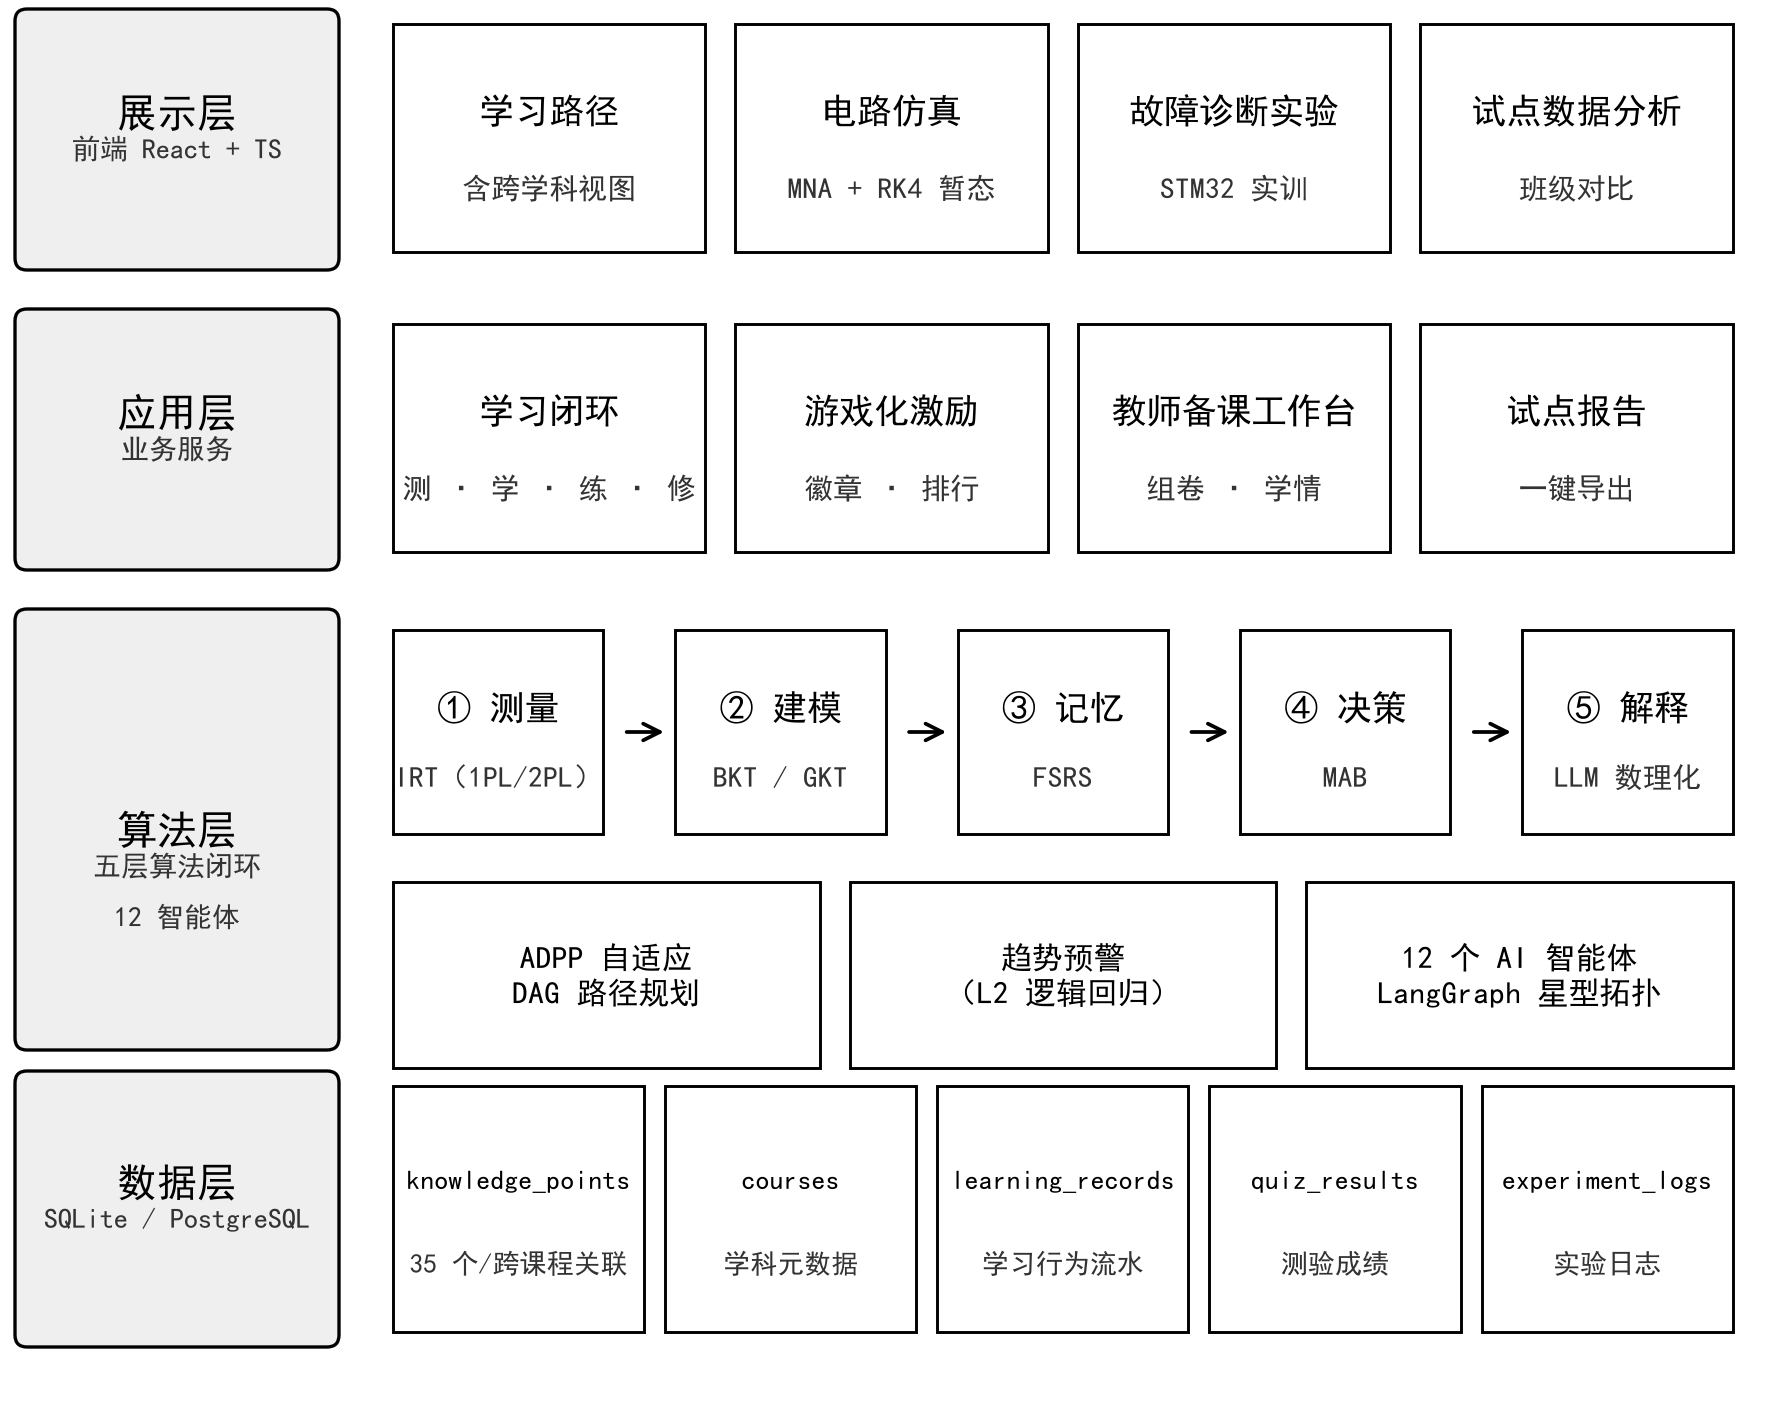
\includegraphics[width=15cm]{arch.png}\end{center}
\subsection{（二）技术选型依据}
\begin{longtable}{|p{7.5cm}|p{7.5cm}|}
\hline
\textbf{技术} & \textbf{选型理由（与学科需求对应）} \\ \hline
\endfirsthead
\hline
\textbf{技术} & \textbf{选型理由（与学科需求对应）} \\ \hline
\endhead
React 18 + TypeScript & 交互式实验实训界面（电路拖拽/仿真/可视化）需要高交互性能与类型安全 \\ \hline
Ant Design 5 & 教育工具的企业级组件体系，信息密度优先 \\ \hline
FastAPI + SQLAlchemy & 异步高性能 API，支撑 WebSocket 流式辅导 \\ \hline
LangGraph & 多智能体编排框架，星型拓扑匹配教育角色体系 \\ \hline
SQLite → PostgreSQL & 开发/试点轻量部署，可平滑迁移 \\ \hline
讯飞星火/DeepSeek 等多模型 & 5 家 LLM 统一接口 + 自动降级，教学场景成本可控 \\ \hline
\end{longtable}
\subsection{（三）核心技术模块}
\subsubsection{1. 多智能体协同（12 Agent，LangGraph 星型拓扑）}


12 个智能体按教育角色划分：课程设计师（Supervisor）、画像师、路径规划师、资源生成师、辅导助手五个核心角色负责主链路；知识图谱构建师、思维溯源师支撑知识体系；错误捕捉师负责代码分析；项目拆解师、角色匹配师、协作督导、成果评估师覆盖团队协作场景。智能体之间走标准化的 AgentMessage 通信协议，并带有\textbf{反思循环}（执行-评估-修正，最多 3 次，由 \texttt{REFLECTION\_ENABLED} 配置启用，评审演示时可现场开启）。

\subsubsection{2. 五层教育算法闭环（学科问题解决新方法）}


平台没有沿用“加权平均分 + 规则阈值”的老办法，而是搭了一套\textbf{五层算法闭环：测量 → 建模 → 记忆 → 决策 → 解释}。每层都有经典文献出处，工程实现全部自研。



\textbf{测量 — IRT 认知诊断}（小样本自动 1PL，数据充分可选 2PL；文献 3-5）：学生能力 θ 替代加权平均分，题目难度 b 替代人工 1-5 分级。



\textbf{建模 — BKT + GKT 知识追踪}（pyBKT EM 估计，文献 1-2；可学习门控图卷积，文献 6-7）：逐知识点掌握概率按学生时间留出评估，指标可一键复现；图结构让邻居知识点的掌握状态影响当前点，传播增益 w≥0 保证单调可解释。



\textbf{记忆 — FSRS 间隔重复调度}（文献 9-11）：真实复习队列 + 记忆可提取性预警，把艾宾浩斯遗忘曲线工程化。



\textbf{决策 — Thompson Sampling 多臂老虎机}（文献 12-14）：用在三处——路径调整策略（回炉/强化/加速/维持，分数段候选集保底）、每日练习选题、资源匹配探索层。



\textbf{解释 — LLM 教学化解释}（自研封装）：把上述算法的输出转述成学生能听懂的辅导语言。



这些算法不是摆出来看的演示件，全部接进了业务链路。IRT θ 接入效果评估掌握度（Φ(θ)·100 百分位，\texttt{mastery\_detail} 可溯源）；IRT b 接入 ADPP 学习成本模型与资源匹配难度适配（\texttt{difficulty\_source} 可区分）；GKT 负责路径上的掌握度传播；MAB 挂在路径调整、选题、匹配三条链路上，收益还能闭环回传；FSRS 把到期知识点自动插到学习路径头部的复习阶段（\texttt{review\_source=fsrs\_due} 可溯源）。算法状态同时注入 tutor / error\_catcher / resource\_generator 三处智能体的 prompt（\texttt{build\_ai\_engine\_context} 共享构建，静默降级）。趋势分析的 6 个因子权重不是人工拍的，由历史数据学习得到（L2 正则逻辑回归，标签取随后一周是否掉队/中断），输出掉队预警概率；样本不足时回退人工先验。

\subsubsection{3. ADPP 自适应 DAG 路径规划（核心自研算法）}


ADPP 的做法是把六样东西组合到一起：关键路径法（CPM）、BKT 掌握度、IRT 难度标定的六因子学习成本模型、加权拓扑排序、自适应阶段划分，以及 Thompson Sampling 动态调整策略，并扩展了跨课程依赖。举个实际的例子：目标知识点是 STM32 定时器 PWM，往前追前置依赖，一路经过 C 语言的位运算、指针，再往前是电路分析的电压波形，系统据此生成一条真正跨学科的学习路径。

\subsubsection{4. 浏览器端 MNA 电路仿真（直流稳态 + RK4 暂态）+ AI 故障诊断（实验实训新范式）}
\begin{itemize}[leftmargin=2em,itemsep=0pt,topsep=0pt]
\item 并查集节点合并（路径压缩+按秩合并）→ MNA 方程组构建 → 列主元高斯消元，全部计算在浏览器端完成，不依赖后端；
\end{itemize}
\begin{itemize}[leftmargin=2em,itemsep=0pt,topsep=0pt]
\item RK4 暂态分析：电容/电感状态变量法 + 四阶 Runge-Kutta 积分，输出充放电波形与稳态建立时间；数值精度经解析解对照验证（RC 指数充电、RL 升流、LC 振荡幅值/周期，\textbf{9/9 通过}）；
\end{itemize}
\begin{itemize}[leftmargin=2em,itemsep=0pt,topsep=0pt]
\item AI 故障诊断实验：3 个故障模板（断路×2 / 短路×1，错值以极端阻值注入实现），学生观察异常测量后选择原因，本地规则判定加 AI 评估（原理讲解/排查方法）；
\end{itemize}
\begin{itemize}[leftmargin=2em,itemsep=0pt,topsep=0pt]
\item 和传统电路实验相比：随时随地、零成本、AI 即时反馈。
\end{itemize}
\subsubsection{5. 跨学科学习链路（学科交叉核心创新）}
\begin{itemize}[leftmargin=2em,itemsep=0pt,topsep=0pt]
\item 9 条跨课程知识关联注入（编程思维→电路建模→嵌入式实现）；
\end{itemize}
\begin{itemize}[leftmargin=2em,itemsep=0pt,topsep=0pt]
\item 学科元数据表（courses）：学科领域、核心环节、交叉说明；
\end{itemize}
\begin{itemize}[leftmargin=2em,itemsep=0pt,topsep=0pt]
\item 跨学科综合路径 + DAG 可视化（按学科着色）；
\end{itemize}
\begin{itemize}[leftmargin=2em,itemsep=0pt,topsep=0pt]
\item 跨学科综合实战项目（智能温控风扇：C语言采样→分压电路→PWM调速）。
\end{itemize}
\subsubsection{6. 防幻觉体系（6 道防线）}


输入过滤 → Prompt 加固 → 结构校验 → 代码校验 → 引用溯源 → LLM 自我纠错。其中①-⑤常驻主管线（\texttt{apply\_guards} 规则守卫，零成本），⑥自我纠错随反思循环生效（\texttt{REFLECTION\_ENABLED} 配置启用）。

\subsubsection{7. 试点数据分析（应用效果验证基础设施）}


学习行为、测验成绩、掌握度趋势、实验参与、功能使用五个维度的数据聚合后，可一键导出试点报告（Markdown），并支持班级对比（实验组 vs 对照组）。

\subsection{（四）核心创新点}


对照“学科问题解决新方法、教学科研新模式、AI 技术应用新场景”三个层面，本作品的创新点及与同类做法的对比：

\begin{longtable}{|p{3.2cm}|p{4.8cm}|p{6.4cm}|}
\hline
\textbf{层面} & \textbf{创新点} & \textbf{与同类做法的对比} \\ \hline
\endfirsthead
\hline
\textbf{层面} & \textbf{创新点} & \textbf{与同类做法的对比} \\ \hline
\endhead
学科问题解决新方法 & 五层教育算法闭环（IRT 测量→BKT/GKT 建模→FSRS 记忆→MAB 决策→LLM 解释）与 ADPP 跨学科 DAG 路径规划，把“学什么、先学什么”从教师经验判断变成按认知数据计算 & 主流 AI 学习产品把大模型直接当问答器，没有认知建模层，答不了“为什么给这个学生推这个知识点”；本作品每条推荐可溯源到算法状态（mastery\_detail、difficulty\_source 等字段可查） \\ \hline
教学科研新模式 & 12 个教育角色智能体覆盖备课、学习、实训、纠错、协作、学情全流程；教师端实时学情与试点报告把期末“经验总结”变成过程性“数据研究” & 传统 LMS 只负责内容分发，学情到期中考试才可见；市面智能辅导产品多聚焦单点答疑，不覆盖教学全环节 \\ \hline
AI 技术应用新场景 & 浏览器端 MNA+RK4 电路仿真叠加 AI 故障诊断；跨课程知识关联（C 语言→电路→嵌入式）生成跨学科学习路径；综合实战项目贯通三门课 & 传统仿真器只输出数值结果，不解释异常原因；同类学习平台多作用于单一课程，缺少跨学科链路 \\ \hline
\end{longtable}


三个层面的共同基础是 AI 技术与学科特色的深度适配：算法层全部选用教育测量与学习科学的经典模型（IRT/BKT/GKT/FSRS 均有明确文献出处）而非通用推荐算法，内容层由电子信息工程专业成员把关学科正确性，场景层直接对应教学实践、实验实训、自主学习、教学管理四类真实环节。

\section{四、方案可行性}
\subsection{（一）技术可行性}


全栈技术都是工业级开源方案（React / FastAPI / LangGraph），没有用不可控的黑盒组件。算法部分（ADPP 路径规划、IRT/BKT/GKT/FSRS/MAB 五层算法引擎、趋势权重学习器、MNA+RK4 电路求解器）全部源码在仓库内，公式与文献出处见附录参考文献。



团队技术能力与这套技术栈是对口的：队长为电子信息工程专业，课程训练覆盖 C 语言、电路分析、单片机开发，独立完成后端 39 个 API 模块与五层算法引擎的实现；全栈代码、测试脚本与部署运维均由团队自己完成（分工见五（三）），不存在“方案写得出来、代码拿不出来”的脱节。



测试方面，所有可复现脚本随仓库交付：算法层专项断言 \textbf{116 项全部通过}（覆盖 BKT/IRT/FSRS/MAB/GKT/NCD/时间留出评估/五层接线/趋势学习器/匹配探索/安全与接线加固）；API 全链路冒烟 38 项（用演示库真实数据训练 IRT/GKT/趋势学习器）；后端 \textbf{210 个路由 0 崩溃}，AIC 功能回归 29 项、数据流 23 项、Agent/LLM 专项 23 项全部通过；前端 E2E 49 个用例（7 个文件），MNA 数值验证 9/9（RC/RL/LC 对照教科书解析解）；前端构建 TypeScript + Vite 零错误。



可靠性这块是吃过亏才补齐的课：早期版本没配 LLM Key 时后端启动直接崩，后来加了降级兜底才稳住。现在是三层保障：5 家 LLM 自动降级链、LLM 故障时的业务降级（引导提示/本地图谱兜底）、限流与防幻觉/安全过滤。逻辑都不复杂，但演示现场最怕的就是这种低级故障。



部署形态也已经过真实环境验证：系统目前运行在腾讯云服务器（OpenCloudOS，2 核 4G）上，Nginx 反向代理 + HTTPS（Let's Encrypt 证书自动续期），后端由 systemd 托管并配置了内存上限与自动重启，日志层接入 journald 轮转。演示站点 https://www.dreamlast.cn 已稳定服务，最近一轮全系统测试期间 \textbf{24 小时零 500 错误}。

\subsection{（二）经济可行性}
\begin{longtable}{|p{3.2cm}|p{4.8cm}|p{6.4cm}|}
\hline
\textbf{成本类别} & \textbf{明细} & \textbf{估算} \\ \hline
\endfirsthead
\hline
\textbf{成本类别} & \textbf{明细} & \textbf{估算} \\ \hline
\endhead
一次性部署 & 云服务器（2核4G） & ¥1,500-2,000/年（学生优惠更低） \\ \hline
LLM API & 讯飞星火（教学场景，100 学生） & ¥300-500/月（开发者有免费额度） \\ \hline
运维 & 学生团队志愿维护 + 开源工具 & ¥0 \\ \hline
对比传统 & 电路实验室建设 & ¥50,000-200,000（仅设备） \\ \hline
对比传统 & 商业 LMS 平台年费 & ¥30,000-100,000/年 \\ \hline
\end{longtable}


算下来，LearnLab 单校部署年成本约 ¥5,000-8,000，比传统实验室和商业平台低一个量级，配合免费额度还能再压。

\subsection{（三）推广价值}
\begin{itemize}[leftmargin=2em,itemsep=0pt,topsep=0pt]
\item 学科内容与平台架构是解耦的：新增一门学科只需要补充知识点 DAG 和内容库，Agent 框架与算法直接复用，目前已用 3 门课程验证过这套机制；
\end{itemize}
\begin{itemize}[leftmargin=2em,itemsep=0pt,topsep=0pt]
\item 落地按三阶段走：先在本校计算机/电子专业试点，再到省内同类院校推广，最后开放学科内容模板，支持 10+ 学科接入；
\end{itemize}
\begin{itemize}[leftmargin=2em,itemsep=0pt,topsep=0pt]
\item 全部验证脚本（算法断言、全路由冒烟、功能回归）与试点报告工具随仓库交付，外校引入后可独立复现测试与效果评估，不依赖原团队；
\end{itemize}
\begin{itemize}[leftmargin=2em,itemsep=0pt,topsep=0pt]
\item LLM 依赖做了风险隔离：支持 5 家 LLM 切换与自动降级；电路仿真、知识图谱、游戏化等非 LLM 核心功能不依赖任何 API。
\end{itemize}
\section{五、项目实施}
\subsection{（一）实施计划}
\begin{longtable}{|p{2.6cm}|p{2.6cm}|p{4.2cm}|p{4.6cm}|}
\hline
\textbf{阶段} & \textbf{时间} & \textbf{内容} & \textbf{交付物 / 验收口径} \\ \hline
\endfirsthead
\hline
\textbf{阶段} & \textbf{时间} & \textbf{内容} & \textbf{交付物 / 验收口径} \\ \hline
\endhead
需求分析与学科界定 & 第 1-2 周 & 学科痛点调研、学科定位（计算机+电子信息） & 需求分析文档；学科-环节-痛点清单（3 环节 9 条） \\ \hline
系统架构设计 & 第 3 周 & 技术选型、架构分层、智能体角色设计 & 架构设计文档；12 智能体角色与 AgentMessage 协议定义 \\ \hline
核心模块开发 & 第 4-10 周 & 12 Agent、ADPP 算法、MNA 仿真、前端体系 & 五层算法引擎与 ADPP 代码入库；MNA 求解器过解析解对照；前端页面全量可用 \\ \hline
测试与优化 & 第 11-12 周 & E2E 测试、性能/安全测试 & E2E 49 用例、算法专项断言 116 项全绿；210 路由冒烟 0 崩溃 \\ \hline
AIC 功能增强 & 第 13-15 周 & 跨学科链路、故障诊断实验、试点数据采集、多模型降级 & 9 条跨课程关联上线；3 类电路故障实验；5 家 LLM 降级链 \\ \hline
小规模试点 & 第 15-16 周 & 8 名学生（实验组 4 + 对照组 4）试用 + 前后测 + 问卷 & 前后测对比与试点数据分析报告（教师端一键导出） \\ \hline
文档与提交 & 第 17 周 & 技术方案、测试报告、演示材料 & 全套参赛交付材料，验证脚本随源码可复现 \\ \hline
\end{longtable}
\subsection{（二）资源保障}
\begin{itemize}[leftmargin=2em,itemsep=0pt,topsep=0pt]
\item 硬件：开发笔记本×3、云服务器 1 台（试点部署）；
\end{itemize}
\begin{itemize}[leftmargin=2em,itemsep=0pt,topsep=0pt]
\item 软件：全部开源/免费（React/Vite/FastAPI/SQLite/Playwright）；
\end{itemize}
\begin{itemize}[leftmargin=2em,itemsep=0pt,topsep=0pt]
\item LLM API：讯飞星火开发者免费额度 + DeepSeek 低成本 API；
\end{itemize}
\begin{itemize}[leftmargin=2em,itemsep=0pt,topsep=0pt]
\item 资金：开发与试点期近零成本（全部开源软件 + LLM 免费额度；规模化部署的单校年成本约 ¥5,000-8,000，明细见四（二）经济可行性）。
\end{itemize}
\subsection{（三）团队协作（跨专业组队）}


三名成员来自三个专业，分别对应平台的三个核心侧面：马其瑞负责算法引擎与后端（电子信息工程的 C 语言、电路、嵌入式课程训练，保证电路与 STM32 内容的学科正确性），孙雨瑶负责试点数据与统计分析（数据科学训练保证效果验证可信度），居欣月负责可视化与文档交付（GIS 的空间可视化与制图训练直接用于 DAG 知识图谱与学情图表）。

\begin{longtable}{|p{2.6cm}|p{3.0cm}|p{4.4cm}|p{5.0cm}|}
\hline
\textbf{成员} & \textbf{照片} & \textbf{专业方向} & \textbf{角色定位} \\ \hline
\endfirsthead
\hline
\textbf{成员} & \textbf{照片} & \textbf{专业方向} & \textbf{角色定位} \\ \hline
\endhead
马其瑞\newline 队长 2025 级 & 
\includegraphics[height=3.2cm]{mqr.jpg} & 电子信息工程 & 后端架构与教育算法引擎；学科内容正确性把关；生产环境部署运维 \\ \hline
孙雨瑶\newline 2025 级 & 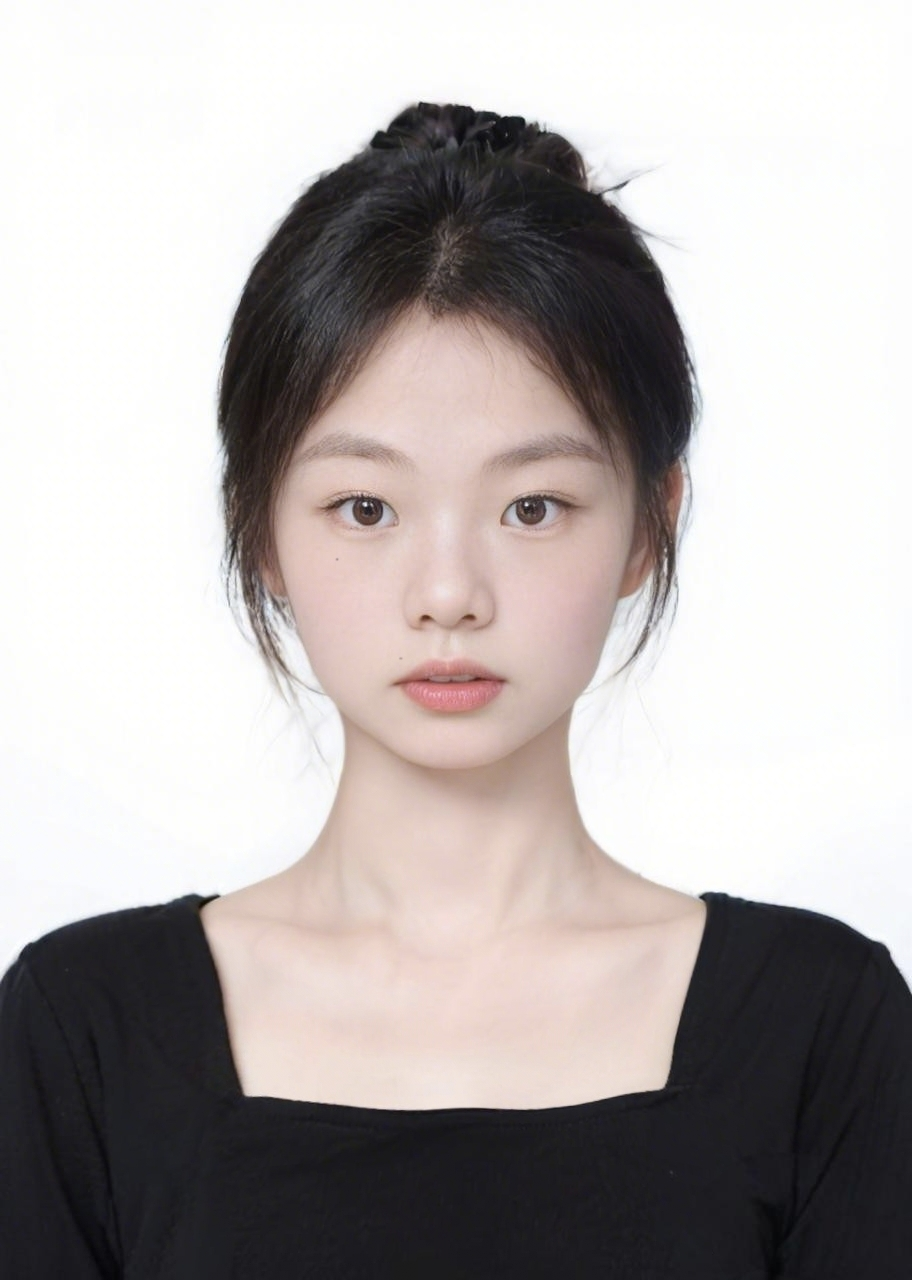
\includegraphics[height=3.2cm]{syy.jpg} & 数据科学与大数据技术 & 试点组织实施与数据质量把关；功能与数据流测试验证 \\ \hline
居欣月\newline 2025 级 & 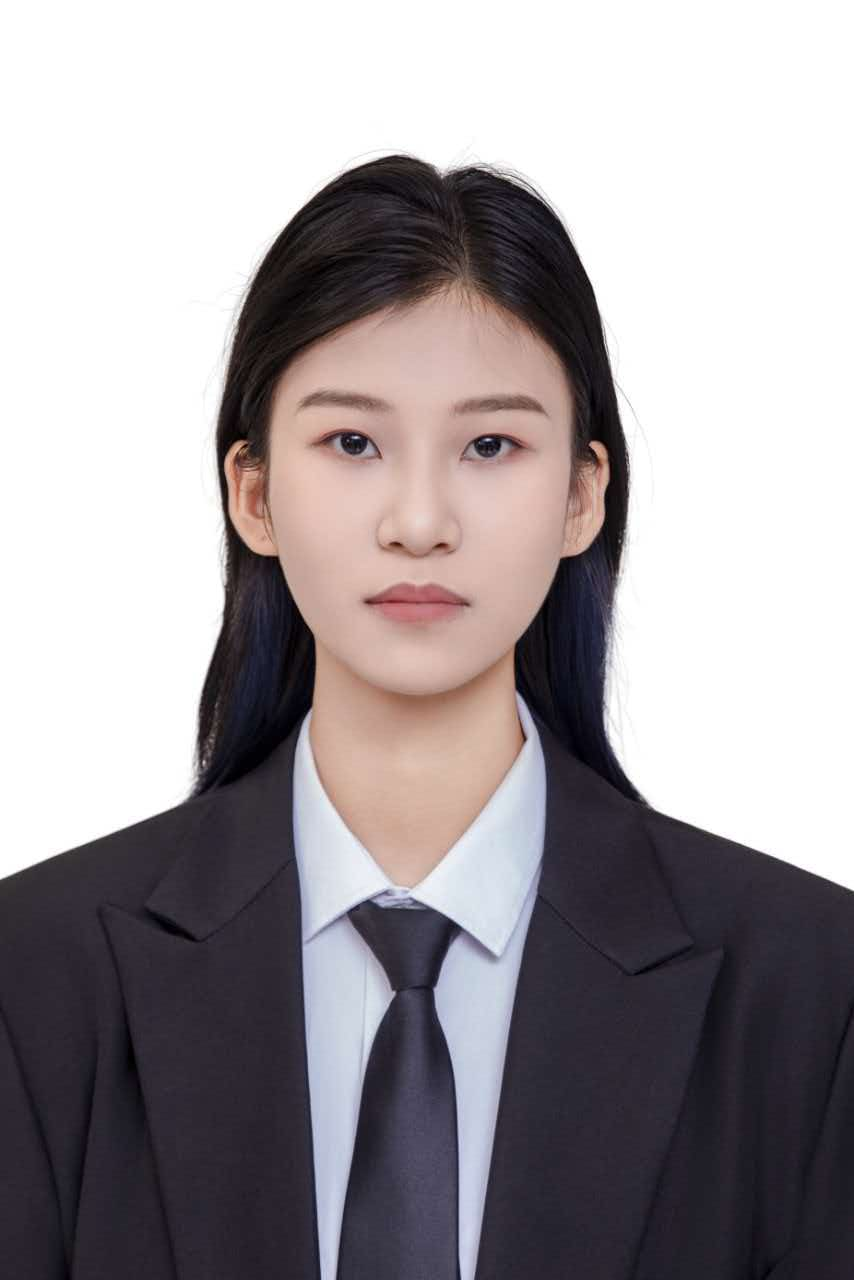
\includegraphics[height=3.2cm]{jxy.jpg} & 遥感科学与技术（GIS 方向） & 前端页面与数据可视化开发；参赛材料排版与交付 \\ \hline
\end{longtable}


各成员的模块划分、任务清单与完成情况如下。

\subsubsection{1. 马其瑞：后端架构与算法引擎}


电子信息工程专业的课程训练覆盖 C 语言、电路分析、单片机开发，与平台主打的“C 语言—电路—嵌入式”学科内容对口，因此由其承担技术底座与学科内容正确性两条线，共五个模块：

\begin{longtable}{|p{3.2cm}|p{4.8cm}|p{6.4cm}|}
\hline
\textbf{模块} & \textbf{具体任务} & \textbf{完成情况} \\ \hline
\endfirsthead
\hline
\textbf{模块} & \textbf{具体任务} & \textbf{完成情况} \\ \hline
\endhead
系统架构 & FastAPI 分层后端（39 个 API 模块）与 SQLite 数据模型设计，覆盖学习、测验、诊断、协作、教师端全业务线 & 已上线运行；210 个路由冒烟测试 0 崩溃 \\ \hline
教育算法引擎 & IRT/BKT/GKT/FSRS/MAB 五层闭环与 ADPP 路径规划引擎的实现、调参与离线评估 & 算法专项断言 116 项全部通过；按学生维度做时间留出评估，输出 AUC/LogLoss/Brier 及基线对照 \\ \hline
智能体编排 & LangGraph 12 智能体调度、AgentMessage 通信协议、执行-评估-修正的反思循环 & 全部就位；反思循环最多 3 次、支持配置开关，评审时可现场演示 \\ \hline
学科内容工程 & “C 语言—电路—STM32”课程内容与题库建设；浏览器端电路仿真 MNA 求解器；C 代码静态分析器 & MNA 数值验证 9/9，RC/RL/LC 结果与教科书解析解一致；错误捕捉覆盖典型语法与逻辑错误 \\ \hline
生产部署运维 & 腾讯云部署（www.dreamlast.cn）、HTTPS 证书自动续期、进程守护、LLM 降级兜底 & 线上持续运行，提交前实测 24 小时零 500 错误；未配置 LLM Key 时自动降级，演示不中断 \\ \hline
\end{longtable}
\subsubsection{2. 孙雨瑶：试点数据与质量验证}


数据科学专业的训练核心是统计实验设计与数据清洗，对应平台“有没有效果、数据可不可信”的证据线，共五个模块：

\begin{longtable}{|p{3.2cm}|p{4.8cm}|p{6.4cm}|}
\hline
\textbf{模块} & \textbf{具体任务} & \textbf{完成情况} \\ \hline
\endfirsthead
\hline
\textbf{模块} & \textbf{具体任务} & \textbf{完成情况} \\ \hline
\endhead
测评工具设计 & 前测试卷、后测试卷、学习体验问卷、知情同意书的编制 & 全套定稿，随试点材料交付 \\ \hline
试点组织实施 & 招募电子信息专业大一学生 8 名，分实验组（SY01-SY04）与对照组（CK01-CK04）；制定前测→平台学习→后测→问卷的流程 & 试点于 9 月 26 日启动，两组学生按流程推进，行为数据自动落库 \\ \hline
数据质量把关 & IRT/BKT 训练数据的清洗规则、作答有效性核验、匿名编号管理 & 清洗与核验规则定稿；试点数据回收后执行前后测对比与效度分析 \\ \hline
功能测试验证 & AIC 功能回归 29 项、数据流 23 项、真实环境 HTTP 22 项的测试执行 & 全部通过；测试脚本随仓库交付，可一键复现 \\ \hline
行为数据埋点 & 学习行为事件设计（观看/阅读/练习/复习/完成/跳过/重置），支撑学习时长与路径差异统计 & 已上线运行，行为流水自动落库 \\ \hline
\end{longtable}
\subsubsection{3. 居欣月：前端页面与数据可视化}


遥感科学与技术（GIS 方向）的专业核心是空间数据的组织与可视化表达，负责把算法输出转成学生与教师“看得懂、愿意用”的界面，共五个模块：

\begin{longtable}{|p{3.2cm}|p{4.8cm}|p{6.4cm}|}
\hline
\textbf{模块} & \textbf{具体任务} & \textbf{完成情况} \\ \hline
\endfirsthead
\hline
\textbf{模块} & \textbf{具体任务} & \textbf{完成情况} \\ \hline
\endhead
学生端页面 & 学习中心、学习路径、AI 辅导、知识库、知识树、错题诊断、资源中心、个人空间等 10 个页面 & 全部完成；24 个页面逐页遍历零 JS 错误、零横向溢出 \\ \hline
教师端页面 & 教学仪表盘、班级对比、学情预警、试点数据分析报告等 14 个页面 & 全部完成，试点报告支持一键导出 \\ \hline
数据可视化 & 跨学科 DAG 知识图谱、学情趋势图表、排行榜、成就徽章墙 & 已上线；GIS 的空间布局与制图训练直接用于知识图谱的层次表达 \\ \hline
交互质量保障 & 移动端适配、学习中心布局调优、新用户引导流程 & 前端 E2E 49 个用例（7 个文件）通过；构建 TypeScript + Vite 零错误 \\ \hline
材料排版交付 & 技术方案 PDF 排版（md→HTML→PDF 管线）、佐证材料整理、源码包验收 & 已交付；系统运行佐证截图 13 张随材料提交 \\ \hline
\end{longtable}


协作机制上，团队用 Git 版本控制（main 保护分支 + 提交审核）和任务看板管理，每周例会同步进度；跨专业模块之间靠 API 接口契约协作，前端按接口文档并行开发，数据侧按埋点口径独立取数，互不阻塞。三个专业各管一段，人员结构本身就贴合“AI 技术 × 学科场景”，也是对赛道“避免技术与学科场景脱节”要求的组织层面回应。

\section{六、应用效果}
\subsection{（一）应用效果预期}


平台对学科核心环节的改善是可预期的，且每一项都设计了对应的验证方式，不以主观描述为准。

\begin{longtable}{|p{3.2cm}|p{4.8cm}|p{6.4cm}|}
\hline
\textbf{维度} & \textbf{预期效果} & \textbf{验证方式} \\ \hline
\endfirsthead
\hline
\textbf{维度} & \textbf{预期效果} & \textbf{验证方式} \\ \hline
\endhead
学习效率 & ADPP 路径规划减少无效学习时间（预估 20-30\%）：零基础学生不再面对超出能力的题目，有基础学生跳过已掌握内容 & 前后测对比 + 学习时长统计 \\ \hline
个性化程度 & 画像驱动的资源/路径适配，同一个班里不同基础的学生拿到不同的学习顺序与资源 & 系统使用日志分析（路径差异率） \\ \hline
实验实训 & 电路故障诊断正确率、实验完成度提升；虚拟环境试错零成本 & experiment\_logs 统计 \\ \hline
教师效率 & 备课与组卷从小时级降到分钟级，学情从期中滞后变为实时洞察 & 教师端使用记录 + 访谈 \\ \hline
\end{longtable}


其中学习效率一项的来源要说明：ADPP 把学生按掌握度分配到不同的路径分支，减少的是“在已掌握知识点上重复练习”的时间；这部分节省随学生基础差异浮动，试点后会用实测数据修正预估。

\subsection{（二）试点方案（已启动）}


试点平台已部署上线（https://www.dreamlast.cn，腾讯云 2 核 4G + Nginx + HTTPS）。材料都先行备齐：知情同意书、前后测问卷（微信小程序发放）、匿名编号规则。8 名电子信息专业大一学生（实验组 SY01-SY04、对照组 CK01-CK04）已招募到位，流程如下：

\begin{itemize}[leftmargin=2em,itemsep=0pt,topsep=0pt]
\item 流程：前测 → 实验组使用 LearnLab 学习 1-2 周（要求完成一次“标记完成”和一次 AI 辅导提问，累计 10-15 分钟）→ 后测 → 反馈问卷
\end{itemize}
\begin{itemize}[leftmargin=2em,itemsep=0pt,topsep=0pt]
\item 数据采集：系统自动采集（学习行为/测验/实验参与/功能使用）+ 前后测成绩 + 用户问卷
\end{itemize}
\begin{itemize}[leftmargin=2em,itemsep=0pt,topsep=0pt]
\item 分组意义：对照组按传统方式自学同样内容，两组后测对比即可分离出平台本身的贡献
\end{itemize}
\begin{itemize}[leftmargin=2em,itemsep=0pt,topsep=0pt]
\item 报告：试点数据分析页自动生成（含前后测对比、实验参与分布、功能使用 Top），导出后作为应用效果佐证
\end{itemize}
\subsection{（三）算法效果验证设计（“传统 vs 算法”可量化对照）}


平台内置了一批能直接产出对照数据的验证点，试点期间自动落库，避免“只有代码验证、没有效果数据”：

\begin{longtable}{|p{2.2cm}|p{2.2cm}|p{2.6cm}|p{3.4cm}|p{3.0cm}|}
\hline
\textbf{对照点} & \textbf{传统方法} & \textbf{算法方法} & \textbf{可量化指标} & \textbf{当前状态} \\ \hline
\endfirsthead
\hline
\textbf{对照点} & \textbf{传统方法} & \textbf{算法方法} & \textbf{可量化指标} & \textbf{当前状态} \\ \hline
\endhead
掌握度测量 & 最近 5 次加权平均分 & IRT θ 百分位（Φ(θ)·100） & 两口径逐生逐日差值、与后测成绩的效度相关 & 已接线，演示库 8 学生实测 \\ \hline
路径成本 & 人工 1-5 难度分级 & IRT 标定 b 值连续插值 & 同知识点两来源耗时差、路径总时长变化 & 已接线，difficulty\_source 可区分 \\ \hline
知识追踪 & 无（画像快照） & BKT EM 估计 & 时间留出 AUC / LogLoss / Brier（并与最近正确率、多数类比较） & 已上线；小样本结果附置信区间与风险提示 \\ \hline
掌握度传播 & 逐点独立 & GKT 图卷积传播 & 图感知掌握度 vs 逐点掌握度对后测的预测增益 & 已训练（可学习门控） \\ \hline
记忆调度 & 统一间隔复习 & FSRS 个性化调度 & 到期知识点复习完成率、可提取性分布 & 已上线 \\ \hline
路径调整策略 & 50/70/90 固定规则 & Thompson Sampling（规则先验冷启动） & strategy\_source 分组的提分统计 & 已接线，收益闭环回传 \\ \hline
选题与资源推荐 & 固定顺序/人工权重 & MAB 探索-利用 & 各臂收益曲线、资源类型点击/完成率 & 已接线 \\ \hline
\end{longtable}


试点结束后，这七个对照点能回答两个问题：平台有没有用，以及效果来自哪一个算法环节。第二个问题更要紧，归因证据是同类产品普遍缺失的。

\subsection{（四）功能验证数据（系统可用性）}
\begin{itemize}[leftmargin=2em,itemsep=0pt,topsep=0pt]
\item 算法层专项断言 116 项全部通过（覆盖 BKT/IRT/FSRS/MAB/GKT/NCD/时间留出评估/五层接线/趋势学习器/匹配探索）
\end{itemize}
\begin{itemize}[leftmargin=2em,itemsep=0pt,topsep=0pt]
\item API 全链路冒烟 38 项（演示库真实数据训练 IRT/GKT/趋势学习器并验证端到端输出）
\end{itemize}
\begin{itemize}[leftmargin=2em,itemsep=0pt,topsep=0pt]
\item 后端 210 个路由 0 崩溃；AIC 功能回归 29 项、数据流 23 项、Agent/LLM 专项 23 项、真实环境 HTTP 22 项全部通过
\end{itemize}
\begin{itemize}[leftmargin=2em,itemsep=0pt,topsep=0pt]
\item 前端 E2E 49 个用例（7 文件）+ MNA 数值验证 9/9（RC/RL/LC 对照解析解）
\end{itemize}
\begin{itemize}[leftmargin=2em,itemsep=0pt,topsep=0pt]
\item 提交前全系统实测 3 轮：24 个页面逐页遍历（学生 10 页 + 教师 14 页）零 JS 错误、零横向溢出；API 全接口 26 项通过（含越权访问 403 校验）；新用户注册→引导问卷→路径生成→成就解锁 11 步全旅程零异常；生产环境 24 小时零 500
\end{itemize}
\begin{itemize}[leftmargin=2em,itemsep=0pt,topsep=0pt]
\item 全部验证脚本随仓库交付，可一键复现
\end{itemize}
\subsection{（五）成果展示（佐证索引）}
\begin{itemize}[leftmargin=2em,itemsep=0pt,topsep=0pt]
\item 系统运行截图 13 张（学生端 8 页 + 教师端 4 页 + 登录页）：见佐证材料“系统功能实证”章节
\end{itemize}
\begin{itemize}[leftmargin=2em,itemsep=0pt,topsep=0pt]
\item 测试验证数据摘要表：见佐证材料“测试验证”章节
\end{itemize}
\begin{itemize}[leftmargin=2em,itemsep=0pt,topsep=0pt]
\item 试点前后测与满意度数据：试点结束后由教师端试点报告页导出，补充进佐证材料
\end{itemize}
\begin{itemize}[leftmargin=2em,itemsep=0pt,topsep=0pt]
\item 算法离线评估：backend/reports/algorithm\_evaluation.md（随源码交付）
\end{itemize}
\subsection{（六）佐证材料与提交对照}


官方“效果验证依据”要求的四类证据，对应关系如下：教学试点数据（试点报告 + 前后测，收集中）、系统行为数据（learning\_records/experiment\_logs 自动落库，已就绪）、用户反馈（反馈问卷，随试点回收）、功能验证（上述 116 项断言与全路由冒烟，已完成）。四类证据中三类已就位，试点数据回收后即可形成完整的效果验证闭环。

\section{七、总结与展望}
\subsection{（一）方案总结}


本工作的核心创新集中在五点：



\noindent\hangindent=2em 1.~跨学科学习链路：打通“编程思维→电路建模→嵌入式实现”，含 9 条跨课程知识关联、跨学科路径算法和综合实战项目；



\noindent\hangindent=2em 2.~五层教育算法闭环：IRT 测量 → BKT/GKT（可学习门控）建模 → FSRS 记忆 → MAB 决策 → LLM 解释，全部接进业务链路，并能产出“传统 vs 算法”的对照数据；



\noindent\hangindent=2em 3.~AI 虚拟实验实训：浏览器端 MNA 直流稳态 + RK4 暂态（解析解对照验证），AI 在其上叠加故障诊断与原理讲解；



\noindent\hangindent=2em 4.~多智能体教育角色体系：12 个 Agent 从零设计（不是通用框架套用），覆盖学习闭环全流程；



\noindent\hangindent=2em 5.~可靠性工程：5 模型自动降级、6 道防幻觉防线、LLM 故障时的业务降级。



不足也有几处，如实说：试点数据仍在收集中，应用效果的真实学生量化验证待完善（对照实验设计已就绪，见第六部分）；学科内容目前覆盖 3 门课程，跨学科关联的广度待扩展；电路暂态分析面向线性 RLC 电路（状态变量法），含非线性元件/受控源的电路待扩展；趋势权重学习器依赖趋势快照积累（≥10 个样本方可训练），当前以人工先验权重兜底。

\subsection{（二）未来展望}


新工科的交叉融合还在深化，嵌入式、物联网方向的复合型人才缺口短期内看不到收窄的迹象，这是这套平台持续有用的前提。技术上值得跟进的有两件事：多模态大模型成熟后，电路仿真可以支持“看着波形图直接提问”的视觉化分析；Agent 框架演进到更自主的形态后，辅导智能体会更接近一名随时在场的助教。推广节奏不变：先把本校试点的效果做扎实，再谈省内推广与开放学科模板库（目标覆盖 10+ 学科）。

\section{八、附录}
\subsection{（一）提交材料对照表（官方“作品要求”逐项对应）}
\begin{longtable}{|p{7.5cm}|p{7.5cm}|}
\hline
\textbf{官方要求（三、作品要求 \& 五、技术方案大纲）} & \textbf{本方案对应位置} \\ \hline
\endfirsthead
\hline
\textbf{官方要求（三、作品要求 \& 五、技术方案大纲）} & \textbf{本方案对应位置} \\ \hline
\endhead
明确聚焦学科专业、界定领域场景 & 二（一）学科专业界定 \\ \hline
学科需求分析报告 & 二（二）核心痛点梳理（教学/实验实训/自主学习三环节） \\ \hline
AI 技术应用方案 & （三）解决方案设计（架构/选型/核心模块） \\ \hline
作品功能说明 & 《03\_功能与验证报告》（学生端 9 模块 + 教师端 6 模块逐项说明）；一（二）核心目标表 \\ \hline
效果验证依据 & 六、应用效果（算法对照设计 + 功能验证数据 + 试点方案） \\ \hline
跨专业组队分工与协作机制 & 五（三）团队协作 \\ \hline
创新点及对比传统方式优势 & 一（三）为什么必须用 AI；三（三）2 五层算法闭环；七（一）核心创新 \\ \hline
推广价值与小规模试点案例 & 四（三）推广价值；六（二）试点方案 \\ \hline
代码与模型（可复现性） & 八（二）代码与验证脚本 \\ \hline
参考文献 & 八（三） \\ \hline
学术伦理与知识产权 & 八（四） \\ \hline
\end{longtable}
\subsection{（二）代码与模型}
\begin{itemize}[leftmargin=2em,itemsep=0pt,topsep=0pt]
\item 完整源代码：GitHub 仓库（Vizzi-cyber/A3），Git 提交历史可追溯全部迭代
\end{itemize}
\begin{itemize}[leftmargin=2em,itemsep=0pt,topsep=0pt]
\item 算法层（backend/app/algorithms/，全部自研或文献复现）：
\end{itemize}
\begin{itemize}[leftmargin=2em,itemsep=0pt,topsep=0pt]
\item \texttt{path\_planning\_dag.py} — ADPP 自适应 DAG 路径规划（BKT/IRT/GKT/MAB 四路接线，策略 MAB 决策）
\end{itemize}
\begin{itemize}[leftmargin=2em,itemsep=0pt,topsep=0pt]
\item \texttt{irt\_diagnoser.py} — IRT 1PL/2PL MAP 联合估计（scipy BFGS）
\end{itemize}
\begin{itemize}[leftmargin=2em,itemsep=0pt,topsep=0pt]
\item \texttt{bkt\_engine.py} — pyBKT 完整贝叶斯知识追踪（EM 参数估计 + AUC 验证）
\end{itemize}
\begin{itemize}[leftmargin=2em,itemsep=0pt,topsep=0pt]
\item \texttt{gkt\_engine.py} — 可学习门控图卷积（自监督 MSE 训练，w≥0 单调约束）
\end{itemize}
\begin{itemize}[leftmargin=2em,itemsep=0pt,topsep=0pt]
\item \texttt{memory\_scheduler.py} — FSRS 间隔重复调度（复习队列/可提取性/持久化）
\end{itemize}
\begin{itemize}[leftmargin=2em,itemsep=0pt,topsep=0pt]
\item \texttt{bandit\_selector.py} — Thompson Sampling 选题器（mabwiser 封装）
\end{itemize}
\begin{itemize}[leftmargin=2em,itemsep=0pt,topsep=0pt]
\item \texttt{ncd\_diagnoser.py} — 神经认知诊断（numpy 向量化实现，单调约束）
\end{itemize}
\begin{itemize}[leftmargin=2em,itemsep=0pt,topsep=0pt]
\item \texttt{trend\_analysis.py} — 多因子趋势分析 + TrendWeightLearner 掉队预警学习器（L2 逻辑回归）
\end{itemize}
\begin{itemize}[leftmargin=2em,itemsep=0pt,topsep=0pt]
\item \texttt{weighted\_matching.py} — 多维加权匹配 + MAB 探索层
\end{itemize}
\begin{itemize}[leftmargin=2em,itemsep=0pt,topsep=0pt]
\item \texttt{effect\_evaluation.py} — 学习效果评估（IRT θ 掌握度 + FSRS 记忆小节）
\end{itemize}
\begin{itemize}[leftmargin=2em,itemsep=0pt,topsep=0pt]
\item 电路仿真（frontend/src/pages/circuit-simulator/utils/mna-solver.ts）：并查集 + MNA 直流稳态 + 状态变量法 RK4 暂态，数值经解析解对照验证
\end{itemize}
\begin{itemize}[leftmargin=2em,itemsep=0pt,topsep=0pt]
\item 训练/验证脚本（backend/scripts/，一键复现）：\texttt{verify\_ai\_algorithms.py}（算法断言）、\texttt{evaluate\_algorithms.py}（按学生时间留出，输出 AUC/LogLoss/Brier/置信区间及基线对照）、\texttt{verify\_p0\_wiring\_api.py}（38 项 API 全链路）、\texttt{verify\_aic\_features.py}（29 项回归）、\texttt{verify\_all\_routes.py}（210 路由冒烟）、\texttt{verify\_dataflow.py} 等
\end{itemize}
\begin{itemize}[leftmargin=2em,itemsep=0pt,topsep=0pt]
\item 训练端点：\texttt{POST /algorithms/irt/fit}、\texttt{/algorithms/bkt/fit}、\texttt{/algorithms/gkt/train}、\texttt{/algorithms/trend/train}（启动时自动拟合 BKT/IRT）
\end{itemize}
\begin{itemize}[leftmargin=2em,itemsep=0pt,topsep=0pt]
\item 数据注入脚本：seed\_cross\_discipline.py（跨学科关联）、seed\_classes.py（班级）
\end{itemize}
\subsection{（三）参考文献}


\textbf{教育算法（按五层闭环顺序）：}



\noindent\hangindent=2em 1.~Corbett, A. T., \& Anderson, J. R. (1995). Knowledge tracing: Modeling the acquisition of procedural knowledge. \textit{User Modeling and User-Adapted Interaction}, 4(4), 253–278.（BKT）



\noindent\hangindent=2em 2.~Badrinath, A., Wang, F., \& Pardos, Z. A. (2021). pyBKT: An Accessible Python Library of Bayesian Knowledge Tracing Models. \textit{Proceedings of the 14th International Conference on Educational Data Mining (EDM 2021)}.



\noindent\hangindent=2em 3.~Rasch, G. (1960). \textit{Probabilistic Models for Some Intelligence and Attainment Tests}. University of Chicago Press.（Rasch 模型/IRT 1PL）



\noindent\hangindent=2em 4.~Lord, F. M. (1980). \textit{Applications of Item Response Theory to Practical Testing Problems}. Routledge.（IRT 2PL）



\noindent\hangindent=2em 5.~Baker, F. B., \& Kim, S.-H. (2004). \textit{Item Response Theory: Parameter Estimation Techniques} (2nd ed.). Marcel Dekker.（MAP 联合估计）



\noindent\hangindent=2em 6.~Nakagawa, H., Iwasawa, Y., \& Matsuo, Y. (2019). Graph-based Knowledge Tracing: Modeling Student Proficiency Using Graph Neural Network. \textit{IEEE/WIC/ACM International Conference on Web Intelligence (WI 2019)}.（GKT）



\noindent\hangindent=2em 7.~Kipf, T. N., \& Welling, M. (2017). Semi-Supervised Classification with Graph Convolutional Networks. \textit{International Conference on Learning Representations (ICLR 2017)}.（GCN/拉普拉斯归一化）



\noindent\hangindent=2em 8.~Wang, F., Liu, Q., Chen, E., Li, Z., Qi, G., \& Shang, J. (2020). Neural Cognitive Diagnosis for Intelligent Education Systems. \textit{AAAI 2020}.（NCD）



\noindent\hangindent=2em 9.~Ye, J., Su, J., \& Cao, Y. (2022). A Stochastic Shortest Path Algorithm for Optimizing Spaced Repetition Scheduling. \textit{Proceedings of the 28th ACM SIGKDD Conference on Knowledge Discovery and Data Mining (KDD 2022)}.（FSRS）



\noindent\hangindent=2em 10.~Liu, R., et al. (2023). Optimizing Spaced Repetition Schedule by Capturing the Dynamics of Memory. \textit{IEEE Transactions on Knowledge and Data Engineering (TKDE)}.（FSRS 记忆动力学）



\noindent\hangindent=2em 11.~open-spaced-repetition. py-fsrs: Free Spaced Repetition Scheduler (Python). https://github.com/open-spaced-repetition/py-fsrs



\noindent\hangindent=2em 12.~Russo, D. J., Van Roy, B., Kazerouni, A., Osband, I., \& Wen, Z. (2018). A Tutorial on Thompson Sampling. \textit{Foundations and Trends in Machine Learning}, 11(1), 1–96.（Thompson Sampling）



\noindent\hangindent=2em 13.~Clement, B., Roy, D., Oudeyer, P.-Y., \& Lopes, M. (2015). Multi-Armed Bandits for Intelligent Tutoring Systems. \textit{Journal of Educational Data Mining}, 7(2), 20–39.（MAB 选题/ZPDES）



\noindent\hangindent=2em 14.~Fidelity Center for Applied Technology. Mabwiser: An ARD Library for Multi-Armed Bandits. https://github.com/fidelity/mabwiser



\noindent\hangindent=2em 15.~Ebbinghaus, H. (1885/1913). \textit{Memory: A Contribution to Experimental Psychology}. Teachers College, Columbia University.（遗忘曲线）



\textbf{教育学与政策：}



\noindent\hangindent=2em 16.~Bloom, B. S. (1984). The 2 Sigma Problem: The Search for Methods of Group Instruction as Effective as One-to-One Tutoring. \textit{Educational Researcher}, 13(6), 4–16.



\noindent\hangindent=2em 17.~VanLehn, K. (2011). The Relative Effectiveness of Human Tutoring, Intelligent Tutoring Systems, and Other Tutoring Systems. \textit{Educational Psychologist}, 46(4), 197–221.



\noindent\hangindent=2em 18.~中华人民共和国教育部. (2017). 教育部办公厅关于开展新工科研究与实践的通知（“新工科建设”复旦共识/天大行动系列）.



\noindent\hangindent=2em 19.~中华人民共和国教育部. (2018). 高等学校人工智能创新行动计划.



\noindent\hangindent=2em 20.~中华人民共和国教育部. (2018). 教育信息化 2.0 行动计划.



\textbf{技术框架文档：}



\noindent\hangindent=2em 21.~LangGraph 官方文档. https://langchain-ai.github.io/langgraph/



\noindent\hangindent=2em 22.~邱关源, 罗先觉. (2018). 《电路》（第 6 版）. 高等教育出版社.（节点电压法/MNA）

\subsection{（四）知识产权、学术伦理与其他材料}


知识产权方面：平台代码全部自研，无知识产权争议；第三方组件均为开源许可（React/TypeScript/FastAPI/LangGraph 为 MIT，Ant Design 为 MIT，pyBKT 为 BSD-3，py-fsrs 为 MIT，mabwiser 为 BSD-3，NumPy/SciPy 为 BSD，Playwright 为 Apache-2.0）；LLM 服务通过官方 API 合规调用（讯飞星火/DeepSeek 等），不涉及模型权重分发。



教学内容与规范方面：课程知识的组织对齐现行课程教学大纲与主流教材体系（电路部分以邱关源《电路》（第 6 版）为参照，见参考文献 22），不复制受版权保护的教材原文；题库与讲义内容经电子信息工程专业成员核对，符合学科教学规范。学术伦理方面：试点数据采集遵循知情同意（试点前发放知情同意书），学生可随时退出；数据采集遵循最小化原则，仅采集学习行为、成绩、功能使用等教学必需数据，不采集个人敏感信息；学生数据仅用于本教学试点的效果分析，报告输出做匿名化与聚合处理；不将任何未实际发生的试点结果表述为已完成。



其他佐证材料：测试说明书（12 章，系统测试佐证）、试点知情同意书（试点前发放）、演示视频（3-5 分钟，覆盖跨学科路径、故障实验、算法对照面板、教师报告）。

\end{document}
